\documentclass[letterpaper, landscape]{exam}
\usepackage{2in1, lscape} 
\printanswers

\usepackage{units} 
\usepackage[fleqn]{amsmath}
\usepackage{float}
\usepackage{mdwlist}
\usepackage{booktabs}
\usepackage{caption}
\usepackage{fullpage}
\usepackage{enumerate}
\usepackage{graphicx}
\usepackage[justification=justified]{caption}

\setcounter{tocdepth}{1}
\everymath{\displaystyle}

\author{}
\date{\today}
\title{Calculus I \\ Week Fifteen}

\begin{document}

  \maketitle
  \tableofcontents
  \section{Homework 13} % (fold)
  \label{sec:Homework 13}

  When finding the second derivative using implicit differentiation, make sure to go back and plug
  in the first derivative in the answer. Answer key didn't do this.
  
  \section{Section 4.1} % (fold)
  
  \subsection{Minimum/Maximum} % (fold)

  \begin{itemize}
    \item absolute min/max is smallest/largest $f(x)$ in the domain
    \item Local max at $x = a$ means for all $b$ in some open interval around $a$, $f(a) > f(b)$
  \end{itemize}

  \subsection{Extreme Value Theorem} % (fold)
  
  If $f$ is continuous on closed interval $[a, b]$ then it has a maximum and minimum in that
  interval.

  Continuous and closed matter because you might have a vertical asymptote or undefined value where
  \[
    \lim_{x \to a} f(a) = L
  \]

  but $f(a)$ isn't defined so there is no maximum
  
  \subsection{Fermat's Theorem} % (fold)
  
  two ways of saying it:
  \begin{itemize*}
    \item If $f$ has a local min/max at $c$ and $f'(c)$ exists, then $f'(c) = 0$ 
    \item If $f$ has a local min/max at $c$ then $f'(c) = 0$ or $f'(c)$ doesn't exist.
    \item If $f$ has a local min/max at $c$ then $c$ is a critical number
  \end{itemize*}

  Values where $f'(c) = 0$ or $f'(c)$ is not defined are {\em critical numbers}.

  \begin{itemize*}
    \item Draw local max with $f'$ exists and $f'$ doesn't exist.
    \item Draw $f(x) = x^3$ where $f'(0) = 0$ and there is no min/max at $x = 0$
    \item Draw $f(x) = \frac{1}{x}$ where $f'(0)$ doesn't exist and there is no min/max at $x = 0$
  \end{itemize*}

  \subsection{Absolute Maximums} % (fold)
  
  To find absolute min/max for a continuous function on a closed interval, 

  \begin{itemize*}
    \item find all the critical numbers
    \item evaluate $f$ at all the critical numbers and endpoints
    \item largest value is max and smallest value is min
  \end{itemize*}

  \subsection{Examples} % (fold)

  \begin{description}

    \item[49] $f(x) = 2x^3 - 3x^2 -12x + 1$; $[-2, 3]$
      \begin{solution}
        \begin{tabular}[H]{rr}
          \toprule
          $x$ & $f(x)$ \\
          \midrule
          $-2$  & $-3$ \\
          $-1$  & $8$ \\
          $2$   & $-19$ \\
          $3$   & $-8$ \\
          \bottomrule
        \end{tabular}
      \end{solution}

      \begin{figure}[H]
        \centering
        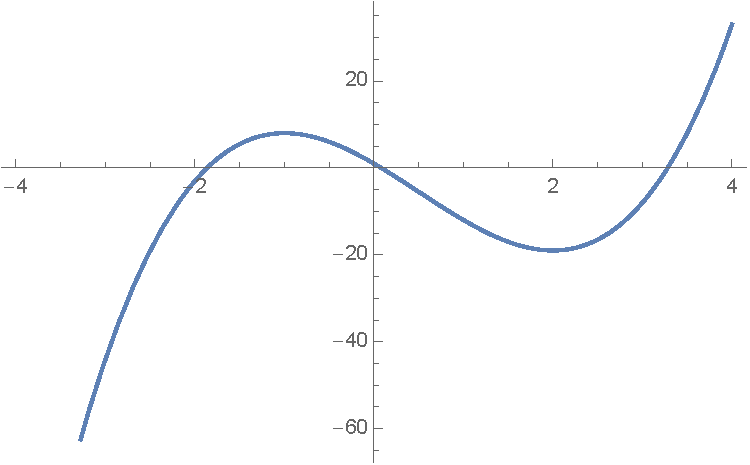
\includegraphics[scale = 0.6]{ex41_49.pdf}
        \caption{Exercise 49}
        \label{fig:ex41_49}
      \end{figure}

    \item[54]
      $f(x) = \frac{x^2 - 4}{x^2 + 4}$ $[-4, 4]$

      \begin{solution}
        $f'(x) = \frac{16x}{\left(x^2 + 4\right)^2}$

        \begin{tabular}[H]{rr}
          \toprule
          $x$  & $f(x)$ \\
          \midrule
          $-4$ & $\frac{3}{5}$ \\
          $0$  & $-1$ \\
          $4$  & $\frac{3}{5}$ \\
          \bottomrule
        \end{tabular}

        \begin{figure}[H]
          \centering
          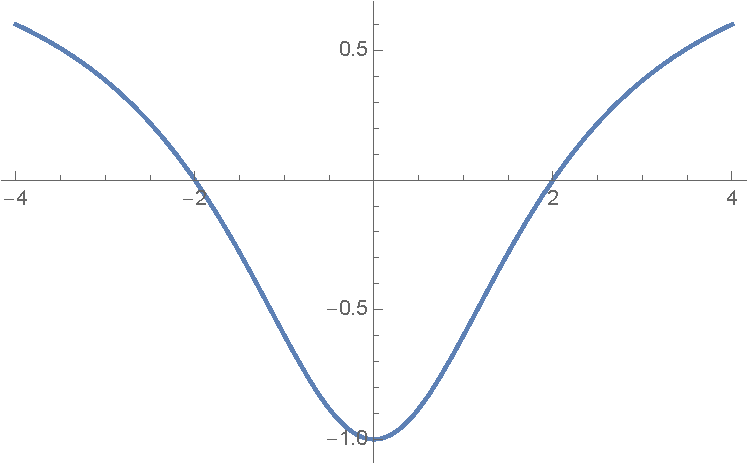
\includegraphics[scale = 0.6]{ex41_54.pdf}
        \caption{Exercise 54}
        \label{fig:ex41_54}
        \end{figure}
      \end{solution}

  \end{description}

  \section{Section 4.3} % (fold)
  
  \subsection{First Derivative} % (fold)
  
  \begin{itemize*}
    \item $f$ is increasing when $f'(x) > 0$
    \item $f$ is decreasing when $f'(x) < 0$
    \item min/max may occur when $f'(x) = 0$
  \end{itemize*}

  First derivative test for min/max:

  \begin{quote}
    If $f'$ changes sign at a critical number, $c$ then $c$ is a local min/max. If $f'$ doesn't change
    sign at $c$ then $c$ isn't a local min/max.
  \end{quote}

  \subsection{Second Derivative} % (fold)
  
  \subsubsection{Concavity} % (fold)
  
  \begin{itemize*}
    \item If $f''(x) > 0$ for all $x$ in an interval, then $f$ is {\em concave upward} in the
      interval
    \item If $f''(x) < 0$ for all $x$ in an interval, then $f$ is {\em concave downward} in the
      interval
  \end{itemize*}

  \subsubsection{Min/Max} % (fold)
  \begin{itemize*}
    \item If $f(c) = 0$ and $f''(c) > 0$ (concave upward), then $f(c)$ is a local minimum
    \item If $f(c) = 0$ and $f''(c) < 0$ (concave downward), then $f(c)$ is a local maximum
  \end{itemize*}

  If $f''(c) = 0$ it doesn't help tell whether or not $f(c)$ is a local min/max.
  
  \newpage

  \subsection{Examples} % (fold)
  
  \begin{description}
    \item[36]
      \begin{align*}
        f(x)   & = x^4 + 8x^3 + 200 \\
        f'(x)  & = 4x^2 (x + 6) \\
        f''(x) & = 12x (x + 4) \\
      \end{align*}

      \begin{itemize*}
        \item Critical numbers are $x = 0$ and $x = 6$
        \item $f''(x) > 0$ when $x < -4$ or $x > 0$
        \item $f'(x) < 0$ when $x < -6$ and $f'(x) > 0$ when $x > -6$, so $f(-6) = -232$ is a local
          minimum
        \item $f''(-6) > 0$ $f(-6)$ is a local minimum
      \end{itemize*}

      \begin{figure}[H]
        \centering
        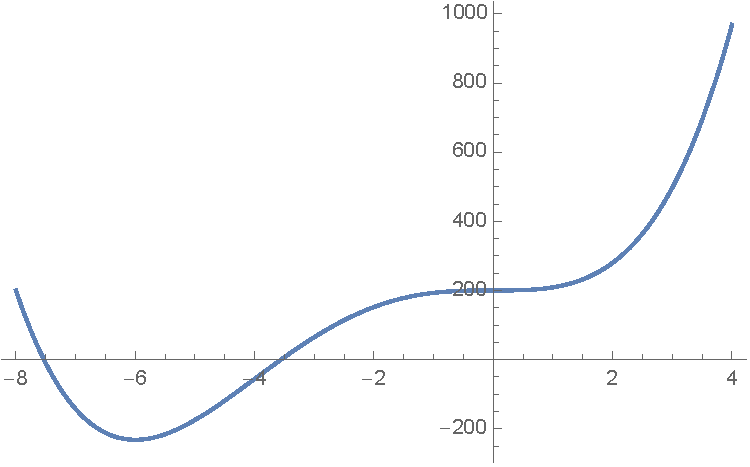
\includegraphics[scale = 0.6]{ex43_36.pdf}
        \caption{Exercise 36}
        \label{fig:ex_4.3_36}
      \end{figure}
      
    \newpage

    \item[10]
      \begin{align*}
        f(x)   & = 4x^3 + 3x^2 -6x + 1 \\
        f'(x)  & = 12x^2 + 6x - 6 \\
        f''(x) & = 24x + 6 \\
      \end{align*}

      \begin{itemize*}
        \item Critical numbers are $x = -1$ and $x = \frac{1}{2}$ 
        \item $f'(x) > 0$ when $x < -1$ or $x > \frac{1}{2}$
        \item $f''(x) > 0$ when $x > - \frac{1}{4}$ 
        \item local max at $(-1, 6)$
        \item local min at $\left( \frac{1}{2}, - \frac{3}{4} \right)$
      \end{itemize*}

      \begin{figure}[H]
        \centering
        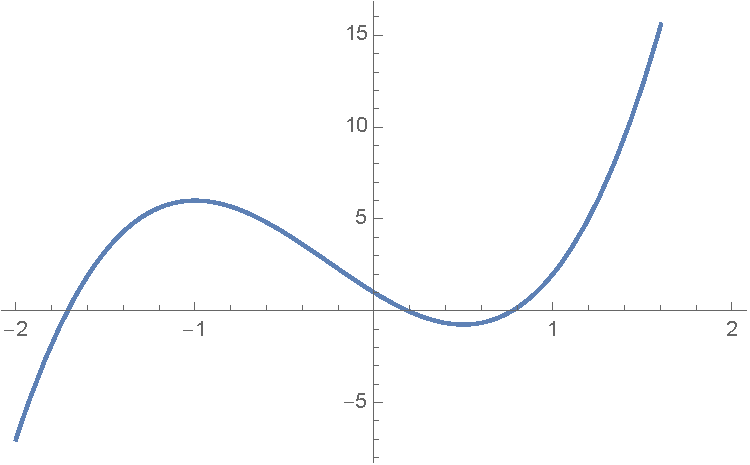
\includegraphics[scale = 0.6]{ex43_10.pdf}
        \caption{Exercise 10}
        \label{fig:ex_4.3_10}
      \end{figure}

    \newpage

    \item[19]
      \begin{align*}
        f(x)   & = x^5 - 5x + 3 \\
        f'(x)  & = 5x^4 -5 \\
        f''(x) & = 20x^3 \\
      \end{align*}

      \begin{itemize*}
        \item Critical numbers are $x = \pm 1$ 
        \item $f'(x) > 0$ when $x < -1$ or $x > 1$
        \item $f''(x) > 0$ when $x > 0$
        \item local min at $(1, -1)$
        \item local max at $(-1, 7)$
      \end{itemize*}

      \begin{figure}[H]
        \centering
        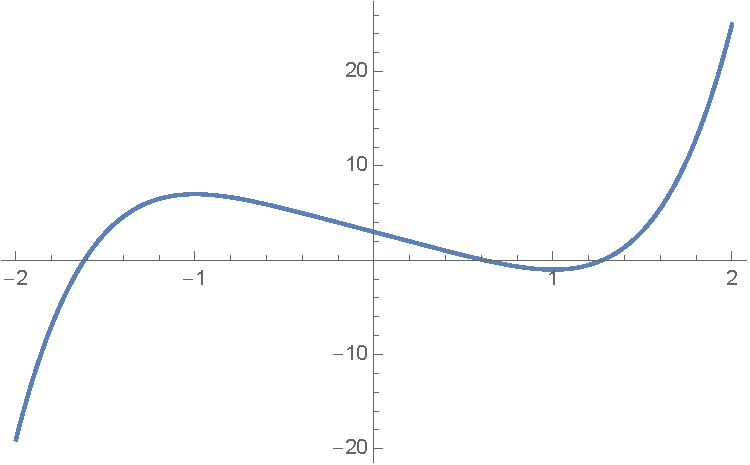
\includegraphics[scale = 0.6]{ex43_19.pdf}
        \caption{Exercise 19}
        \label{fig:ex_4.3_19}
      \end{figure}

    \newpage

    \item[12]
      \begin{align*}
        f(x)   & = \frac{x^2}{x^2 + 3} \\
        f'(x)  & = \frac{6x}{\left(x^2 + 3\right)^2} \\
        f''(x) & = \frac{ 18 - x^2 }{ \left(x^2 + 3 \right)^3 } \\
      \end{align*}

      \begin{itemize*}
        \item Critical number is $x = 0$ 
        \item $f'(x) > 0$ when $x > 0$ 
        \item $f''(x) > 0$ when $-1 < x < 1$ 
        \item local min at $(0, 0)$
        \item no local max
      \end{itemize*}

      \begin{figure}[H]
        \centering
        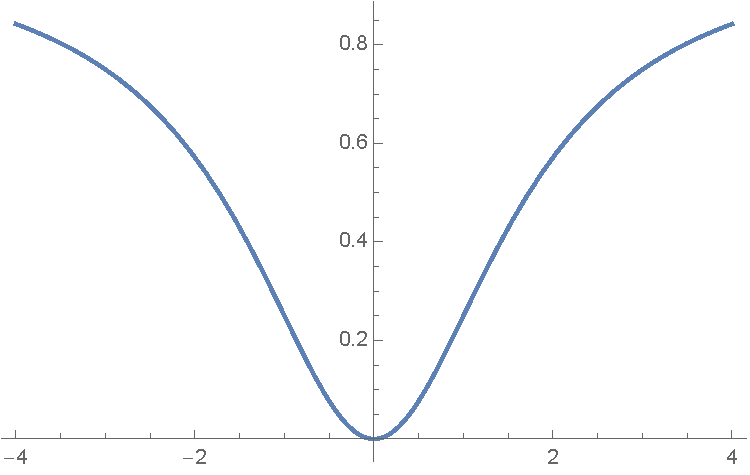
\includegraphics[scale = 0.6]{ex43_12.pdf}
        \caption{Exercise 12}
        \label{fig:ex_4.3_12}
      \end{figure}

  \end{description}

\end{document}

